\chapter[General introduction]{General introduction}
\label{ch:intro}

%Coauthorship-----------------------------------------------------------------------------------

\section*{Co-authorship statement}
\addcontentsline{toc}{section}{Co-authorship statement}

Sections of this chapter has been published as:\\

David Wilkins, \textbf{Sheree Yau}, Timothy Williams, Michelle Allen, Mark V. Brown, Matthew Z. DeMaere, Federico M. Lauro and Ricardo Cavicchioli. 
Key Microbial Drivers in Antarctic Aquatic Environments.
\textit{\underline{FEMS Microbiology Reviews}} \\
(doi: 10.1111/1574-6976.12007), 2012.\\

I contributed the section of the publication entitled \emph{Antarctic lakes} excluding the subsection, \emph{Microbial mats as microcosms of Antarctic life}.
This material appears in sections of this introduction.
\newpage

%-----------------------------------------------------------------------------------------------

%\section{Introduction}
Antarctica is a ``frozen desert'' of constant low temperature, little precipitation and is subject to the polar light cycle where only specially adapted organisms can survive.
The continent is covered by ice up to 4 km thick that spans 13.8 million km$^2$.
A tiny 0.32\% of the land area is ice-free, most of which consists of exposed rocky peaks or nunataks such as in the Ellsworth, the Transantarctic and the North Victoria Land Mountains. %figure of continent
Only 1--2\% of that ice-free land is found in coastal oases; however, it is these regions where Antarctic life is concentrated \cite{Hodgson2012}.
They are breeding sites for large animals such as seals, penguins and sea birds and some of the only locations where plants and lichens are found.
Coastal oases are also distinguished by the presence of hundreds of lakes and ponds.
Life in these lakes is microbially dominated with few, if any, metazoan inhabitants \cite{Laybourn-Parry1997} making them ideal locations to study Antarctic microbiota. 
The lakes span a continuum of environmental factors such as salinity and are ``natural laboratories'' to examine adaptations to a property of interest. 
The reduced biodiversity of Antarctic lakes makes them ideal model systems to examine microbial influence on geochemistry as it is possible to encompass a large proportion of the diversity present using molecular methods and relate taxa to particular processes \cite{Laybourn-Parry2007}.

This introduction will review molecular-based microbiological research on Antarctic lakes.
%Add in references to other papers on the lakes in general
As this thesis focused on planktonic communities from two lakes in the Vestfold Hills, emphasis will be given to describing research from this study site and to microbial ecology of the water column.

%---------------------------------------------------------------------------------------------

\section{Antarctic lakes}
%create a map of the regions you want to describe, like in the review paper.
In Antarctica, perenially available liquid water is found predominantly in lakes.
These range from subglacial lakes that are sealed beneath kilometres of ice to completely exposed rock-bound lakes.
The majority of lakes are found in the coastal oases. 
In East Antarctica these include the Vestfold Hills, Bunger Hills, Larsemann Hills, Syowa Oasis, Schirmacher Oasis, Grearson Hills and McMurdo Dry Valleys.
In West Antarctic, the Antarctic Peninsula, the sub-Antarctic islands and maritime islands house multiple lakes. 
Of these locations, the best studied lake systems are those of the McMurdo Dry Valleys, The Vestfold Hills and the sub-Antarctic islands.

These lakes span a wide range of physical and chemical properties from freshwater to hypersaline and constantly ice-covered to melted.
Some are permanently stratified and termed meromictic if they thaw seasonally, or amictic if they are always ice-covered.
Stratified lakes provide a unique opportunity to describe aquatic microbial populations along steep chemical gradients and taxa can be related to the properties of that layer.  
They are also of particular interest because the anoxic bottom waters help preserve a paleogeological record in the sediments of geological and climatic changes.
Most lakes are ice-covered for most of the year making them effectively isolated, and some may be truly closed systems if ice-cover is permanent.
The age of water varies considerably; for example, outflow of subglacial water at Blood Falls is estimated to be 1.5 million years old \cite{Mikucki2009} while water from Lake Miers is less than 300 years old \cite{Green1988}. 

Most of these lakes were formed when the retreat of the continental ice-shelf lead to isostatic uplift of the land \cite{Burton1981}. %check ref
As a result, the majority of lakes in the coastal oases are composed of relic seawater and are predominantly saline or hypersaline \cite{Burke1988}.
In the latter, salinity is high due to concentrated by ablation (evaporation and sublimnation). %ref 
Lakes closer to the coastline may still occasionally experience marine inputs. %ref

Freshwater lakes near the continental ice shelf were likely already above sea-level as the ice receded and are not of marine origin \cite{Bronge1996}. %Laybourn-Parry1992?
Other freshwater lakes were originally marine-derived but have been flushed fresh by glacial meltwater \cite{Pickard1986}.
The chemistry of the exposed lakes is very much influenced by the water balance from local geographic and climatic conditions.
Input sources include precipitation, from the ice-shelf and glacial melt streams \cite{Burton1981}. 

%--------------------------------------------------------------------------------------------

\section{The Vestfold Hills}
The Vestfold Hills \figref{fig:vestfold_map} is a ice-free region of approximately 400 km$^2$ on the eastern shore of the Prydz Bay, East Antarctica in the Australian Antarctic Territory \cite{Gibson1999}.
The region was first sighted and named in 1935 \cite{Law1959}.
Only intermittent expeditions occurred in the area until the establishment of Davis Station (68$^{\circ}$33$'$S, 78$^{\circ}$15$'$E) in 1957 \cite{Law1959}. 
The Vestfold Hills are made up of three large peninsulae, Broad, Mule and Long Peninsula, separated by fjords connected to the sea.
Some of these fjords are large, such as Ellis Fjord, which is 10 km long, up to 100 m deep and has become a stratified system due to its restricted opening to the ocean \cite{Burke1988}.
The region was formed approximately 10,000 years ago in the early Holocene as the continental ice receded and the rocky peninsulae rose above sea-level \cite{Zwartz1998}. 

When first discovered, the Vestfold Hills was immediately noted for its extensive ice-free land and the numerous lakes \cite{Johnstone1973}.
The Australian Antarctic Data Centre lists more than 3,000 water bodies mapped in the Vestfold Hills, ranging in area from 1 to 8,757,944 m$^2$. %check this fact.
\begin{figure}
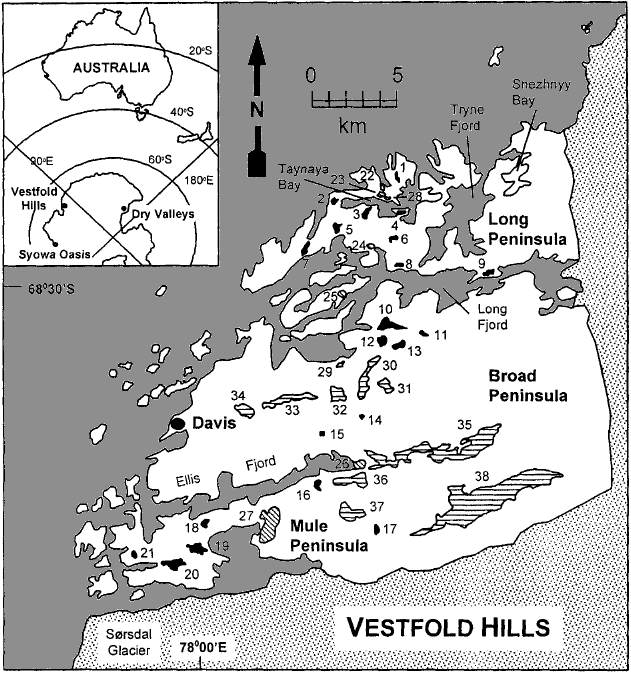
\includegraphics{intro_figures/vestfold_map.png}
\caption[Map of the Vestfold Hills]{A map of the Vestfold Hills showing fjords, bays and lakes (numbered). The Southern Ocean is shown in grey, meromictic lakes coloured in black, seasonally isolated lakes and basins are striped and the continental ice-shelf is stippled. Inset is the position of the Vestfold Hills relative to Australia and to the Antarctic coastal oases. The lakes are: (1) unnamed lake 2, (2) Organic Lake, (3) Pendant Lake, (4) Glider Lake, (5) Ace Lake, (6) unnamed lake 1, (7) Williams Lake, (8) Abraxas Lake, (9) Johnstone Lake, (10) Ekho Lake, (11) Lake Farrell, (12) Shield Lake, (13) Oval Lake, (14) Ephyra Lake, (15) Scale Lake, (16) Lake Anderson, (17) Oblong Lake, (18) Lake McCallum, (19) Clear Lake, (20) Laternula Lake and (21) South Angle Lake. Map image is from \citet{Gibson1999} with some minor modifications.}
\label{fig:vestfold_map}

\end{figure}

More than 300 lakes and ponds have been described, including approximately 20\% of the world's meromictic lakes \cite{Gibson1999}. %check this fact.

%------------------------------------------------------------------------------------------

\section{Insights from molecular studies of Antarctic lakes}
\label{in:insights}
The majority of molecular-based studies of Antarctic lake microbial communities have made use of \ac{PCR} amplification of \ac{SSU} sequences to survey the diversity of \emph{Bacteria} and in some cases \emph{Archaea} and \emph{Eucarya}.
A comprehensive list of PCR-based studies of Antarctic lakes and their major findings are provided in Appendix \ref{app:A}.
It attempts to include all molecular-based studies but some may have been inadvertantly missed.
Microbial composition has been determined by cloning and sequencing of \ac{rRNA} gene amplicons 
\cite{Bowman2000a, Bowman2000b, Gordon2000, Christner2001, Purdy2003, Karr2006, Matsuzaki2006, Kurosawa2010, Bielewicz2011}, 
although many studies have also made use of \ac{DGGE} to provide a molecular ``fingerprint'' of the community 
\cite{Pearce2003a, Pearce2003b, Karr2005, Pearce2005a, Pearce2005b, Unrein2005, Glatz2006, Mikucki2007, Mosier2007, Schiaffino2009, Villaescusa2010}.
Functional genes have also been targeted using \ac{PCR} amplification to assess the potential of biochemical processes occurring, such as nitrogen fixation \cite{Olson1998}, ammonia oxidation \cite{Voytek1999}, anoxygenic photosynthesis \cite{Karr2003}, and dissimilatory sulfite reduction \cite{Karr2005, Mikucki2009}. %add in new studies
These \ac{PCR}-based analyses of Antarctic lake communities have shed light on microbial diversity, temporal and spatial distributions and started to delve into the key drivers in whole ecosystem function.

Relatively few metagenomic studies, which entail random sequencing of environmental \textsc{DNA}, have been published on Antarctic lakes \cite{Lopez-Bueno2009, Ng2010a, Lauro2011, Yau2011}.
However, these few studies have been able to assess both the taxonomic composition and genetic potential of lake communities, and in many cases have linked function to specific members of the community.
When coupled with functional ``-omic'' techniques (to date metaproteomics has been applied, but not metatranscriptomics or stable isotope probing), information has also been gained about the genetic complement expressed by the resident populations \cite{Ng2010a,Lauro2011,Yau2011}.

%------------------------------------------------------------------------------------------
\subsection{Bacterial diversity: adaptation to unique physical and chemical conditions}

Most molecular studies conducted on Antarctic lakes have focused on \emph{Bacteria}.
Consistent with the wide range of physical and chemical properties of Antarctic lakes, a large variation in species assemblages have been found.
While exchange of microorganisms must be able to occur between lakes that are in close vicinity to each other, the data to date indiates that microbial populations are relatively unique to each type of isolated system. 
Nonetheless, certain trends in composition driven by physico-chemical factors and potentially biogeography, are also apparent.
%------------------------------------------------------------------------------------------
\subsubsection{Salinity}
Hypersaline lakes from the Vestfold Hills \cite{Bowman2000b} and McMurdo Dry Valleys \cite{Glatz2006, Mosier2007} were all dominated by \emph{Gammaproteobacteria} and members of the \emph{Bacteroidetes} as well as harboring lower abundance populations of \emph{Alphaproteobacteria}, \emph{Actinobacteria}, and \emph{Firmicutes}.
The surface waters of lakes close to marine salinity resemble marine communities dominated by \emph{Bacteroidetes}, \emph{Alphaproteobacteria} and \emph{Gammaproteobacteria}, but divisions such as \emph{Actinobacteria} and specific clades of \emph{Cyanobacteria} have been found to be overrepresented compared to the ocean \cite{Lauro2011}.
Sediments from saline lakes in the Vestfold Hills \cite{Bowman2000a} and Nuramake-Ike in the Syowa Oasis \cite{Kurosawa2010} were very similar, containing in addition to the surface clades, \emph{Deltaproteobacteria}, \emph{Planctomycetes}, \emph{Spirochaetes}, \emph{Chloroflexi} (green non-sulphur bacteria), \emph{Verrucomicrobia} and representatives of related candidate divisions.
Plankton from freshwater lakes were characterized by an abundance of \emph{Betaproteobacteria}, although \emph{Actinobacteria}, \emph{Bacteroidetes}, \emph{Alphaproteobacteria} and \emph{Cyanobacteria} were also prominent \cite{Pearce2003a, Pearce2005a, Pearce2005b, Schiaffino2009}. 
%------------------------------------------------------------------------------------------
\subsubsection{Trophic status}
Differences in bacterial community structure are also influenced by nutrient availability.
In studies of freshwater lakes in the Antarctic Peninsula and the South Shetland Islands, cluster analysis of \ac{DGGE} profiles grouped together lakes of similar trophic status \cite{Schiaffino2009, Villaescusa2010}.
Most of the variance in community structure could be explained by related chemical parameters such as phosphate and dissolved inorganic nitrogen.
Similarly, three freshwater lakes, Moss, Sombre and Heywood on Signy Island are alike except that Heywood Lake is enriched by organic inputs from seals.
Bacterial composition in each lake changed from winter to summer and this was again correlated to variation in physico-chemical properties \cite{Pearce2005a}. 
The bacterial population of Heywood Lake had shifted from a dominance of \emph{Cyanobacteria} towards a greater abundance of \emph{Actinobacteria} and marine \emph{Alphaproteobacteria} \cite{Pearce2005b}.
This hints at a link between a copiotrophic lifestyle in the Heywood Lake \emph{Actinobacteria} and inhibition of Antarctic freshwater \emph{Cyanobacteria} by eutrophication. 
This type of study exemplifies how inferences can be made about taxa and function by examining population changes over time and over gradients of environmental parameters.
%------------------------------------------------------------------------------------------
\subsubsection{Biogeography}
The relative isolation and diverse chemistries of the lakes facilitates biogeographical and biogeochemical studies. 
The anoxic and sulphidic bottom waters of some meromictic lakes form due to a density gradient that precludes mixing. 
Although sedimentation from the upper aerobic waters may occur, there is little opportunity for interchange of species with the bottom water of lakes allowing for greater divergence in community composition as nutrients can become depleted and products of metabolism can accumulate.
As a result, distinct distributions of bacterial groups can inhabit these strata, and different types of microorganisms can be found in equivalent strata in different lakes. 

A good example of this is the presence of common types of purple sulphur bacteria (\emph{Chromatiales})and \ac{GSB}(\emph{Chlorobi}) in some meromictic lakes and stratified fjords in the Vestfold Hills \cite{Burke1988}, compared to diverse purple non-sulphur bacteria in Lake Fryxell, McMurdo Dry Valleys \cite{Karr2003}. 
%Check if these aren't Roseobacters
In Lake Bonney, the east and west lobes harbor overlapping but distinct communities in the suboxic waters \cite{Glatz2006}.
The east lobe was dominated by \emph{Gammaproteobacteria} and the west lobe by \emph{Bacteroidetes}, illustrating how divergent communities can form from the same seed population. 
In contrast, ice communities are more readily dispersed by wind, aerosols and melt-water. 
16S \ac{rRNA} gene probes designed from bacteria trapped in the permanent ice-cover of Lake Bonney hybridized to microbial mat libraries sourced up to 15 km away \cite{Gordon2000}.
This demonstrates how a single lake may encompass microorganisms that are geographically dispersed, while also harboring others that have restricted niches and are under stronger selection pressure.
%------------------------------------------------------------------------------------------

\subsubsection{Bacterial diversity of Lake Vostok}
Subglacial systems have been isolated from the open environment for hundreds of thousands to millions of years \cite{Siegert2001}.
The biggest of these, Lake Vostok is approximately 4 km below the continental ice-sheet.
As a result they provide a reservoir of microorganisms that may have undergone significant evolutionary divergence from the same seed populations that were not isolated by the Antarctic ice cover. 
To date, molecular microbial studies have concentrated on the accretion ice above the ice-water interface \cite{Priscu1999, Christner2001}.
Accretion ice has been found to contain a low density of bacterial cells from \emph{Alphaproteobacteria}, \emph{Betaproteobacteria}, \emph{Actinobacteria} and \emph{Bacteroidetes} divisions closely allied to other cold environments.
Molecular signatures of a thermophilic \emph{Hydrogenophilus} species were also identified in accretion ice 
raising the possibility that chemoautotrophic thermophiles were delivered to the accretion ice from hydrothermal areas in the lake’s bedrock \cite{Bulat2004, Lavire2006}.

However, interpretation of results from samples sourced from the Lake Vostok bore hole are very challenging as it is difficult to differentiate contaminants from native Vostok microorganisms.
From a study that assessed possible contaminants present in hydrocarbon-based drilling fluid retrieved from the Vostok ice core bore hole, 
six phylotypes were designated as new contaminants \cite{Alekhina2007}. 
Two of these were \emph{Sphingomonas} phylotypes essentially identical to those found in the accretion ice-core \cite{Christner2001},
 which raises question about whether bacteria identified from the ice-cores are representative of Lake Vostok water,
 and is an example of how contamination may occur.
%------------------------------------------------------------------------------------------

\subsection{\emph{Archaea}: methanogens and haloarchaea}
\emph{Archaea} have been detected mainly in anoxic sediments and bottom waters from lakes that range in salinity from fresh to hypersaline.
Those with known isolates are affiliated with methanogens or haloarchaea \cite{Bowman2000a, Bowman2000b, Purdy2003, Kurosawa2010, Lauro2011}.
Anoxia allows for the growth of methanogenic \emph{Archaea} that mineralize fermentation products such as acetate, H$_2$ and CO$_2$ into methane, thereby performing an important step in carbon cycling.
The acetoclastic methanogens thrive in environments where alternative terminal electron acceptors such as sulphate and nitrate have been depleted. 
%This may be why there are none in Organic Lake as there is still sulphate.
One example of this is Lake Heywood where methanogenic \emph{Archaea} were found to comprise 34\% of the total microbial population in the freshwater sediment, the majority of which were \emph{Methanosarcinales}, which include acetate and C1-compound utilizing methanogens \cite{Purdy2003}. 

In general, archaeal populations appear to be adapted to their specific lake environment.
Sediments from saline lakes of the Vestfold Hills were inhabited by members of the \emph{Euryarchaeota} typically found in sediment and marine environments with the phylotypes differing between the lakes examined \cite{Bowman2000a}. 
While a phylotype similar to \emph{Methanosarcina} was identified, the majority were highly divergent. 
Similarly, \emph{Methanosarcina} and \emph{Methanoculleus} were detected in Lake Fryxell but other members of the \emph{Euryarchaeota} and \emph{Crenarchaeota} (a single sequence) were divergent, clustering only with marine clones \cite{Karr2006}. 
Based on the lake chemical gradients and the location of these novel phylotypes in the water column the authors speculated these \emph{Archaea} may be have alternative metabolisms such as anoxic methanotrophy or sulphur-utilization. 

In sediments from Lake Nurume-Ike in the Langhovde region, 205 archaeal clones grouped into three phylotypes, 
with the predominant archaeal clone being related to a clone from Burton Lake in the Vestfold Hills, while the other two did not match to any cultivated species \cite{Kurosawa2010}. 
In hypersaline lakes where bottom waters do not become completely anoxic, methanogens are not present and \emph{Archaea} have extremely low abundance. 
For example, only two archeael clones of the same phylotype were recovered from deep water samples from Lake Bonney \cite{Glatz2006}, 
and Organic Lake in the Vestfold Hills had an extremely low abundance of archaeal clones related to \emph{Halobacteriales} \cite{Bowman2000b}. 
In contrast to these stratified hypersaline lakes, the microbial community in the extremely hypersaline Deep Lake is dominated by haloarchaea \cite{Bowman2000b}. 
Many of the clones identified from Deep Lake are similar to \emph{Halorubrum} (formerly \emph{Halobacterium}) \emph{lacusprofundi} which was isolated from the lake \cite{Franzmann1988}. 


\subsection{\emph{Eucarya} perform multiple ecosystem roles}

Single-celled \emph{Eucarya} are important members of Antarctic aquatic microbial communities.
In many Antarctic systems, eucaryal algae are the main photosynthetic organisms and in others, only heterotrophic protists occupy the top trophic level. 
As eucaryal cells are generally large with characteristic morphologies, microscopic identifications have been used. 
However, microscopy is unable to classify smaller cells such as nanoflagellates with high resolution, although these may constitute a high proportion of algal biomass.
For example, five morphotypes of \emph{Chrysophyceae}, evident in Antarctic lakes were unidentifiable by light microscopy but were able to be classified using \ac{DGGE} and \textsc{DNA} sequencing \cite{Unrein2005}.
Consistent with this, molecular studies specifically targeting eucaryal diversity \cite{Unrein2005, Mosier2007, Bielewicz2011} have identified a much higher level of diversity than previously suspected,
 and the studies have discovered lineages not previously known to be present such as silicoflagellates of the family \emph{Dictyochophyceae} \cite{Unrein2005} and fungi \cite{Mosier2007, Bielewicz2011}.

Most \emph{Eucarya} in Antarctic lakes are photosynthetic microalgae that are present in marine environments with a wide distribution including chlorophytes, haptophytes, cryptophytes and bacillariophytes.
Molecular methods have afforded deeper insight into the phylogenetic diversity within these broader divisions and have revealed some patterns in their distribution. 
Using 18S \ac{rRNA} gene amplification and \ac{DGGE}, the same chrysophyte phylotypes were identified in lakes from the Antarctic Peninsula and King George Island 
despite being 220 km apart \cite{Unrein2005} indicating these species may be well-adapted to Antarctica or highly dispersed.
Similarly, an unknown stramenopile sequence was detected throughout the 18S \ac{rRNA} clone libraries of Lake Bonney 
demonstrating a previously unrecognized taxon occupied the entire photic zone in the lake \cite{Bielewicz2011}. 
In constrast, other groups showed distinct vertical and temporal distributions with cryptophytes dominating the surface, 
haptophytes the midwaters and chlorophytes the deeper layers during the summer while stramenopiles increased in the winter \cite{Bielewicz2011}. 

The influence of flagellates on ecosystem function is not necessarily clear-cut as they can simultaneously inhabit several trophic levels. 
For instance, in Ace Lake the mixotrophic phytoflagellate \emph{Pyramimonas gelidocola} derives a proportion of its carbon intake through bacterivory \cite{Bell2003} but in the nearby Highway Lake, it uptakes dissolved organic carbon \cite{Laybourn-Parry2005}. 
This illustrates potential limitations for deriving ecosystem level functions from taxonomic studies alone, even with taxa that appear physiologically straightforward. 
Further studies are necessary to determine the basis for apparent specific adaptations of some species to particular lakes or lake strata, and for the cosmopolitan distribution of others.
Here, molecular based research of the kind that has been applied to bacteria such as functional gene surveys will undoubtedly help answer these questions.
%add in new studies of photosynthetic genes
%add in the functional gene studies

%--------------------------------------------------------------------------------------------------------------------
%\subsection{Functional gene analyses}
%Several \ac{PCR}-based studies studies have been conducted on lakes from the McMurdo Dry Valleys to determine if potential for vital %biochemical functions are present, rather than determining which taxa are present.
%Nitrogen fixation was examined in Lake Bonney \cite{Olson1998}
%, ammonia oxidation \cite{Voytek1999},

% anoxygenic photosynthesis \cite{Karr2003}, and dissimilatory sulfite reduction \cite{Karr2005, Mikucki2009}.
%This recognising that limited physiological information afforded by PCR-based taxonomic surveys.


%--------------------------------------------------------------------------------------------------------------------
\subsection{Integrative studies to derive whole ecosystem function}
The relatively low diversity of Antarctic microbial food-webs existing within effectively closed systems allows for an integrative understanding of the microbial community and biogeochemical cycling to be obtained. 
This can be achieved by combining molecular information of the taxonomic or functional genes with abiotic parameters or reaction rates.

One such study was conducted on Blood Falls, an outflow of anoxic ferrous brine from the Taylor Glacier in the McMurdo Dry Valleys, where an unusual iron--sulphur cycle was inferred to exist. 
The water is sulphate-rich, exists in permanent darkness and is estimated to have been isolated from external inputs for 1.5 million years \cite{Mikucki2009}. 
16S rRNA gene analysis showed the community was dominated by a close relative of \emph{Thiomicrospira arctica}, an autotrophic sulphur-oxidizing member of the \emph{Gammaproteobacteria} (\emph{Thiotrichales}), as well as sequences related to \emph{Delta}- and \emph{Gammaproteobacteria} capable of iron and/or sulphur compound reduction, and \emph{Bacteroidetes} capable of heterotrophic growth on organic compounds \cite{Mikucki2007}.
A large proportion of adenosine 5$'$-phophosulphate reductase genes related to those involved in dissimilatory sulphate metabolism were detected. 
However, dissimilatory sulphite reductase (\emph{dsrA}) was not present and radioisotope data indicated sulphide is not produced. 
The implication of this is that sulphate reduction does not proceed to sulphide as typically occurs in other aquatic systems, and instead sulphate is expected to be regenerated via an alternative cycle with Fe(III) acting as the terminal electron acceptor \cite{Mikucki2009}. 
This is a fascinating example of how a closed system has adapted to sustain life in the absence of light energy through the use of atypical chemical cycling; a pathway that was speculated to have possibly occurred in the ancient Neoproterozoic ocean (1,000 to 500 mya) \cite{Mikucki2009}.
%describe Allison murray paper.
%--------------------------------------------------------------------------------------------------------------------

\section{`-omics' approaches}
Metagenomics is a powerful tool to explore microbial diversity that permits taxonomic classification and information on genetic content of uncultured taxa in their environment. 
The first large scale metagenomic study of an Antarctic Lake was used to study viruses \cite{Lopez-Bueno2009}
As obligate parasites, viruses cannot be isolated without first having a susceptible host in culture curtailing the possibility of surveying anything but defined viral populations through culture-based techniques.
Viruses do not have a universal gene that may be used as a taxonomic marker, or even universal genetic material so metagenomic sequencing is an ideal approach to understand the viruses.

Analysis of the viral component of the freshwater Lake Limnopolar, Livingston Island uncovered the greatest depth of viral diversity of any aquatic system to date \cite{Lopez-Bueno2009}.
Representatives from 12 viral families were detected, but unlike the two previous viromes that had been published at that time using comparable techniques, ss\textsc{DNA} viruses and large ds\textsc{DNA} viruses that putatively infect \emph{Eucarya} were the dominant viral types. 
The ss\textsc{DNA} viruses were related to circoviruses, geminiviruses, nanoviruses and satellites; viruses previously only known to infect plants and animals indicating they are much more diverse than previously suspected and may constitute new viral families. 
Samples taken in summer showed a shift in the viral community composition towards phycodnaviruses similar to \emph{Ostreococcus tauri} virus, OtV5. 
This shift potentially reflects an increase in the host algae that are stimulated to bloom by the increased light availability.
Subsequent analysis has indicated multiple displacement amplification of low quantities of starting \textsc{DNA} used in virome study leads to a stochastic amplification bias rendering the metagenomes non-quantitative \cite{Yilmaz2010}.
Nonetheless, clear is that viruses perform a crucial role in shaping community structure, driving host evolution and contributing to the dissolved nutrient pool \cite{Danovaro2011} and this first study opened a window to their true diversity and the complexity of incorporating them into a understanding of microbial ecology. 

Motivation for adopting metagenomic and other `-omics' approaches has also stemmed from the inability to obtain physiological data from \ac{PCR}-based taxonomic surveys of environments and limited scope offered by surveys of single functional gene markers.
Although metabolic capacity can often be inferred if there are cultured representatives with the detected genes, close relatives with defined physiologies are often not available.
Inferring functional potential can even be problematic if species or strain level differences exist.
For example, the majority of \emph{Gammaproteobacteria} that have been detected in hypersaline lakes are relatives of \emph{Marinobacter} suggesting that this genus is particularly adapted to hypersaline systems \cite{Bowman2000b, Glatz2006, Matsuzaki2006, Mosier2007}.
Nonetheless, \emph{Marinobacter} species from different lakes appeared biochemically distinct as isolates from hypersaline lake Suribati-Ike were all able to respire \ac{DMSO} but not nitrate \cite{Matsuzaki2006}. 
In contrast, those from the west lobe of Lake Bonney were all able to respire nitrate \cite{Ward1997}. 
Interestingly, in the east lobe of the same lake, nitrate respiration was inhibited although a near-identical \emph{Marinobacter} phylotype was present; it was speculated that the inhibition may have been caused by an as yet unidentified chemical factor \cite{Ward2005, Glatz2006}.
%Similarly \ac{PCR}-based screening of functional genes can determine potential for a microbial process.
%But clear links back to an organism of origin may not be possible if it is highly divergent of horizontally transferred. 
%Furthermore, detection of the gene does not mean that the process is active

An `-omics' approach circumvents the limitations of \ac{PCR} surveys and combined with physico-chemical parameters has the potential to derive an integrative understanding of ecosystem function.
Such an approach, utilising both metagenomics and metaproteomics, was applied to Ace Lake in the Vestfold Hills \cite{Ng2010a, Ng2010b, Lauro2011}. 
The main carbon, nitrogen and sulphur cycles within the stratified water column of Ace Lake was able to be described \cite{Lauro2011}.
A strictly interdependent sulphur cycle was found to exist between \ac{GSB} at the oxycline and \ac{SRB} in the anaerobic zone.
The \ac{GSB} were able to convert sulphide to sulphate but lacked assimilatory sulfate reduction capability \cite{Ng2010a, Ng2010b, Lauro2011}. 
Enzymes involved in dissimilatory sulphate reduction (adenylylsulphate reductase and dissimilatory sulphite reductase) were detected in the metaproteome of the anaerobic zone and linked with \ac{SRB} \cite{Ng2010a, Ng2010b}, completing the dissimilatory sulphur cycle.
It was also apparent that short circuiting of the nitrogen cycle was occurring. 
Nitrogen fixation proteins were not found in the metaproteome, likely due to preferential assimilation of ammonia \cite{Ng2010a, Ng2010b, Lauro2011}.  
Genes involved in nitrification and denitrification were underrepresented indicating the system had shifted away from nitrogen mineralization consistent with a mechanism to conserve bioavailable nitrogen \cite{Lauro2011}. 
It is noteworthy that these findings are in contrast to lakes in the Dry Valleys where ammonia monooxygenase genes were present in the aerobic zone of six lakes of various salinities and extents of stratification \cite{Voytek1999}.
Overall, strong depth partioning, loss of biochemical pathways common in other aquatic systems and the selection of key species were identified as important steps in transiting the microbial population from marine to a meromictic lake ecosystem.

Further results from the study of Ace Lake are presented in Chapter \ref{ch:ace} and metagenomic and metaproteomic analyses of Organic Lake is described in Chapters \ref{ch:olv} and \ref{ch:org}.
%-----------------------------------------------------------------------------------------------------------------

\section{Objectives}
The overall aim of the studies described in this thesis was to explore the microbial communities of Antarctic lakes from an ecosystems level perspective by using metagenomics combined with microscopy, metaproteomics and abiotic datasets.
Ace Lake and Organic Lake, two lakes in the Vestfold Hills, were chosen as the study sites as there are extensive historic environmental records available for these lakes.
As meromictic lakes, differences in the microbial population can be examined along the vertical gradients within the lakes.
Finally, as they are marine-derived systems, comparison between the lake system and the marine environment can be used to identify specific lake adaptations.

The specific objectives of the research were:

\begin{enumerate}
\item 
  To develop epifluorescence microscopy and metaproteomic methodologies to generate independent datasets complementary to metagenomic sequencing.

\item
  To determine the microbial and viral composition of Antarctic lake communities, their functional potential and infer the ecological roles of populations in the community.


\item
  To integrate environmental and biological data to model the lake microbial interactions and geochemical processes.

\end{enumerate}
